% !TEX TS-program = pdflatex
% !TEX encoding = UTF-8 Unicode
\documentclass[12pt]{report}
\usepackage[utf8]{inputenc} % set input encoding (not needed with XeLaTeX)

\usepackage{geometry} % to change the page dimensions
\geometry{a4paper} % or letterpaper (US) or a5paper or....
\geometry{margin=2cm} % for example, change the margins to 2 inches all round

% Packages
\usepackage{pdflscape}
\usepackage{graphicx} % support the \includegraphics command and options
\usepackage[parfill]{parskip} % Activate to begin paragraphs with an empty line rather than an indent
\usepackage{booktabs} % for much better looking tables
%\usepackage{array} % for better arrays (eg matrices) in maths
%\usepackage{paralist} % very flexible & customisable lists (eg. enumerate/itemize, etc.)
%\usepackage{verbatim} % adds environment for commenting out blocks of text & for better verbatim
\usepackage{subfig} % make it possible to include more than one captioned figure/table in a single float
\usepackage{url}

% Headers and Footers
\usepackage{fancyhdr} % This should be set AFTER setting up the page geometry
\pagestyle{fancy} % options: empty , plain , fancy
\renewcommand{\headrulewidth}{0pt} % customise the layout of headers and footers
\lhead{Final Report}\chead{}\rhead{Iain Johnston}
\lfoot{}\cfoot{\thepage}\rfoot{}

% Section Title Appearance
\usepackage{titlesec}
\titleformat{\section}{\large\bfseries}{\thesection}{1em}{\hrule}

% ToC appearance
\usepackage[nottoc,notlof,notlot]{tocbibind} % Put the bibliography in the ToC
\usepackage[titles,subfigure]{tocloft} % Alter the style of the Table of Contents
\renewcommand{\cftsecfont}{\rmfamily\mdseries\upshape}
\renewcommand{\cftsecpagefont}{\rmfamily\mdseries\upshape} % No bold!


% The document content starts below

\title{\textit{Final Report}\\\textbf{Maximising entertainment value in the vote-reveal problem}\\ Final Year Project (CM3203) - 40 Credits}
\author{Author: Iain Johnston (1312579) \\ Supervisor: Richard Booth\\ Moderator: Xianfang Sun}
\date{} % Activate to display a given date or no date (if empty),  otherwise the current date is printed

\begin{document}
\maketitle
\clearpage

\section*{Abstract}

\section*{Acknowledgements}

\tableofcontents %  place a table of contents after the title
\listoffigures
\listoftables
\clearpage % clear the page after the table of contents

%\addcontentsline{toc}{section}{Section z} % how to add an entry to the table of contents that is un-numbered
%\section*{Second Section} % an un-numbered section in the document
%\subsection{A subsection} % an example subsection
\section{Introduction}
% tell the reader what the project is about without assuming special knowledge and without introducing any specific material that might obscure the overview.
% anticipate and combine main points described in more detail in the rest
% include things such as:
% the aim(s) or goal(s) of the project,
% the intended audience or “beneficiaries” of the work done,
% the scope of the project,
% the approach used in carrying out the project,
% assumptions on which the work is based and
% a broad summary of important outcomes.

\section{Background}
% give reader info that they can't be expected to know, but which they need in order to fully understand and appreciate the report
% explain why the project is addressing the problem described in the report
% indicate an awareness of other relevant work
% show clearly that the problem has not been solved by anyone else
% include things such as:
% the wider context of the project,
% the problem that has been identified,
% likely stakeholders within the problem area,
% any theory associated with the problem area,
% any constraints on the approach to be adopted,
% existing solutions relevant to the problem area, and why these are unsuitable or insufficient in this particular case,
% methods and tools that your solution may be based on or use to solve the problem,
% you should also refer to the general problem for which these algorithms are useful (the application(s) for your techniques).
% existing products, documents or artefacts that you should mention could be:
% similar to the one you are proposing,
% support your project,
% your project aims to extend or replace,
% demonstrate the “deficiencies” your project intends to address.

% Your background section should end with a clear statement of the research questions problem your project is trying to answer. 
%These will reflect the aim of your project, but will be different in that they explain the problem you are attempting to solve

\section{Algorithm Designs/Approach}
% give reader a clear picture of the system
% specification becomes: description of the problem and what is required of a solution
% design becomes: description of your approach to solving the problem and your suggested solution(s)
% problem statement section and then a section describing one or more suggested algorithms to solve the problem
% Later in results and evaluations describe how to design experiments to test how well the algorithms solve the problem and present experimental results with an evaluation of your suggested solutions

\section{Implementation of Algorithms}
% describes system but does so at finer level of detail, down to code level
% realisation of concepts and ideas developed earlier
% complete source code should be provided separately
% pick out and describe pieces of code which for example:
% are especially critical in operation of system
% are of particular interest
% illustrate a non-standard or innovative way of implementing an algorithm, data structure
% mention unforeseen problems that you encountered when implementing the system like:
% difficulties involving existing software
% lack of suitable supporting framework
% over ambitious project aims
% A seemingly disproportionate amount of project time can be taken up in dealing with such problems. The Implementation section gives you the opportunity to show where that time has gone.

\section{Results and Evaluation}
% describe to what extent you achieved your goals
% describe how you demonstrate that the system works as intended (or not)
% include comprehensible summaries of the results of all critical test that were carried out
% should try to indicate how confident you are about whatever you have produced, and also suggest what tests would be required to gain further confidence
% describe the reasoning behind the tests to evaluate your results, what tests to execute, what results show and why to execute these tests
% include discussion of how you are designing your experiments to verify hypothesis of more scientifically oriented project
% eg. describe how you compare the performance of your algorithm to other algorithms to indicate better performance and why this is a sound approach. then summarise the results of the tests of experiments
% critically evaluate your results in the light of these tests, describing its strengths and weaknesses. ideas for improvement can be carried over into Future work.
% present a critical appraisal of the project as a whole, including why the programming language and methodology chosen were appropriate

\section{Future Work}
% expressing unrealistic ideas, including what you would have liked to have done if only you had not run out of time
% provide a good starting point for someone else to continue the work which you have begun

\section{Conclusions}
% summary of the aims of the project and a restatement of the main results, i.e. what has been learnt and acheived
% an effective set of conclusions should not introduce new material. Instead it should briefly draw out, summarise, combind and reiterate the main points that have been made in the body of the project report and present opinions based on them

\section{Reflection on Learning}
% identify the impact of what we have done on the assumptions, concepts and ideas we used to make decisions about our work
% try to identify the characteristics of the problem that has been addressed , and consider whether assumptions of decisions about the relevant approach to solving the problem had been appropriate, in order to make a better decision in relation to problems that might be encountered in the future.

\section*{Glossary}
\addcontentsline{toc}{section}{Glossary}  

\section*{Table of Abbreviations}
\addcontentsline{toc}{section}{Table of Abbreviations}

\section*{Appendices}
\addcontentsline{toc}{section}{Appendices}
%\begin{landscape} 
%\section*{Appendix}
%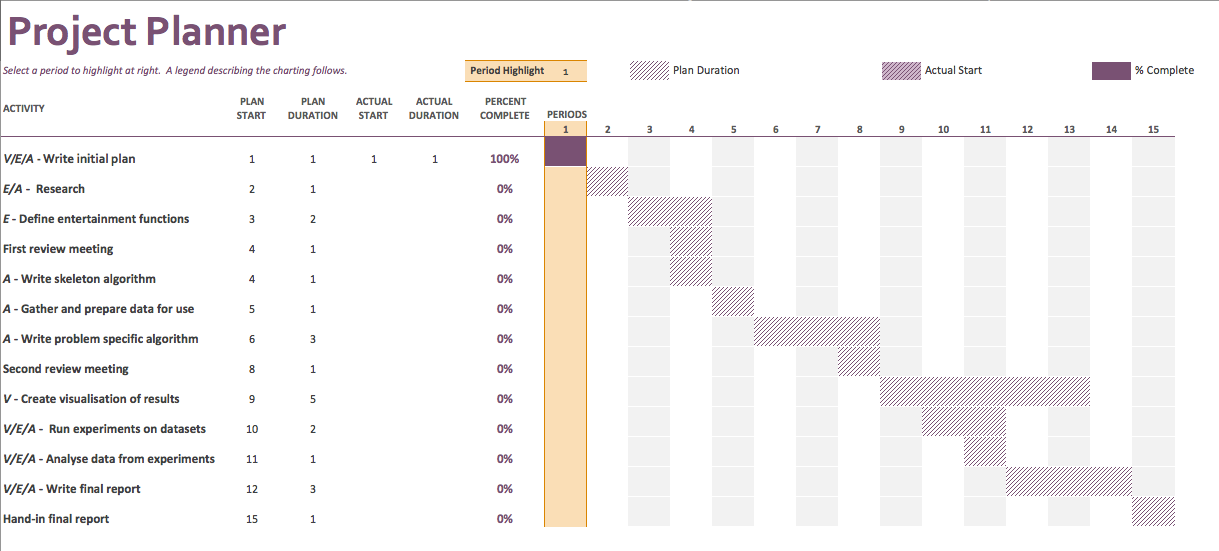
\includegraphics[height=14.5cm, width=\linewidth]{InitialPlanGanttChart.png}
%\end{landscape}

\clearpage
\renewcommand{\bibsection}{\section*{References}}
\addcontentsline{toc}{section}{References}
\bibliography{./References/finalReportBib}{}
\bibliographystyle{ieeetr}

\end{document}
